\documentclass[1p]{elsarticle_modified}
%\bibliographystyle{elsarticle-num}

%\usepackage[colorlinks]{hyperref}
%\usepackage{abbrmath_seonhwa} %\Abb, \Ascr, \Acal ,\Abf, \Afrak
\usepackage{amsfonts}
\usepackage{amssymb}
\usepackage{amsmath}
\usepackage{amsthm}
\usepackage{scalefnt}
\usepackage{amsbsy}
\usepackage{kotex}
\usepackage{caption}
\usepackage{subfig}
\usepackage{color}
\usepackage{graphicx}
\usepackage{xcolor} %% white, black, red, green, blue, cyan, magenta, yellow
\usepackage{float}
\usepackage{setspace}
\usepackage{hyperref}

\usepackage{tikz}
\usetikzlibrary{arrows}

\usepackage{multirow}
\usepackage{array} % fixed length table
\usepackage{hhline}

%%%%%%%%%%%%%%%%%%%%%
\makeatletter
\renewcommand*\env@matrix[1][\arraystretch]{%
	\edef\arraystretch{#1}%
	\hskip -\arraycolsep
	\let\@ifnextchar\new@ifnextchar
	\array{*\c@MaxMatrixCols c}}
\makeatother %https://tex.stackexchange.com/questions/14071/how-can-i-increase-the-line-spacing-in-a-matrix
%%%%%%%%%%%%%%%

\usepackage[normalem]{ulem}

\newcommand{\msout}[1]{\ifmmode\text{\sout{\ensuremath{#1}}}\else\sout{#1}\fi}
%SOURCE: \msout is \stkout macro in https://tex.stackexchange.com/questions/20609/strikeout-in-math-mode

\newcommand{\cancel}[1]{
	\ifmmode
	{\color{red}\msout{#1}}
	\else
	{\color{red}\sout{#1}}
	\fi
}

\newcommand{\add}[1]{
	{\color{blue}\uwave{#1}}
}

\newcommand{\replace}[2]{
	\ifmmode
	{\color{red}\msout{#1}}{\color{blue}\uwave{#2}}
	\else
	{\color{red}\sout{#1}}{\color{blue}\uwave{#2}}
	\fi
}

\newcommand{\Sol}{\mathcal{S}} %segment
\newcommand{\D}{D} %diagram
\newcommand{\A}{\mathcal{A}} %arc


%%%%%%%%%%%%%%%%%%%%%%%%%%%%%5 test

\def\sl{\operatorname{\textup{SL}}(2,\Cbb)}
\def\psl{\operatorname{\textup{PSL}}(2,\Cbb)}
\def\quan{\mkern 1mu \triangleright \mkern 1mu}

\theoremstyle{definition}
\newtheorem{thm}{Theorem}[section]
\newtheorem{prop}[thm]{Proposition}
\newtheorem{lem}[thm]{Lemma}
\newtheorem{ques}[thm]{Question}
\newtheorem{cor}[thm]{Corollary}
\newtheorem{defn}[thm]{Definition}
\newtheorem{exam}[thm]{Example}
\newtheorem{rmk}[thm]{Remark}
\newtheorem{alg}[thm]{Algorithm}

\newcommand{\I}{\sqrt{-1}}
\begin{document}

%\begin{frontmatter}
%
%\title{Boundary parabolic representations of knots up to 8 crossings}
%
%%% Group authors per affiliation:
%\author{Yunhi Cho} 
%\address{Department of Mathematics, University of Seoul, Seoul, Korea}
%\ead{yhcho@uos.ac.kr}
%
%
%\author{Seonhwa Kim} %\fnref{s_kim}}
%\address{Center for Geometry and Physics, Institute for Basic Science, Pohang, 37673, Korea}
%\ead{ryeona17@ibs.re.kr}
%
%\author{Hyuk Kim}
%\address{Department of Mathematical Sciences, Seoul National University, Seoul 08826, Korea}
%\ead{hyukkim@snu.ac.kr}
%
%\author{Seokbeom Yoon}
%\address{Department of Mathematical Sciences, Seoul National University, Seoul, 08826,  Korea}
%\ead{sbyoon15@snu.ac.kr}
%
%\begin{abstract}
%We find all boundary parabolic representation of knots up to 8 crossings.
%
%\end{abstract}
%\begin{keyword}
%    \MSC[2010] 57M25 
%\end{keyword}
%
%\end{frontmatter}

%\linenumbers
%\tableofcontents
%
\newcommand\colored[1]{\textcolor{white}{\rule[-0.35ex]{0.8em}{1.4ex}}\kern-0.8em\color{red} #1}%
%\newcommand\colored[1]{\textcolor{white}{ #1}\kern-2.17ex	\textcolor{white}{ #1}\kern-1.81ex	\textcolor{white}{ #1}\kern-2.15ex\color{red}#1	}

{\Large $\underline{12n_{0131}~(K12n_{0131})}$}

\setlength{\tabcolsep}{10pt}
\renewcommand{\arraystretch}{1.6}
\vspace{1cm}\begin{tabular}{m{100pt}>{\centering\arraybackslash}m{274pt}}
\multirow{5}{120pt}{
	\centering
	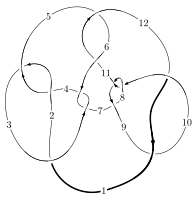
\includegraphics[width=112pt]{../../../GIT/diagram.site/Diagrams/png/2220_12n_0131.png}\\
\ \ \ A knot diagram\footnotemark}&
\allowdisplaybreaks
\textbf{Linearized knot diagam} \\
\cline{2-2}
 &
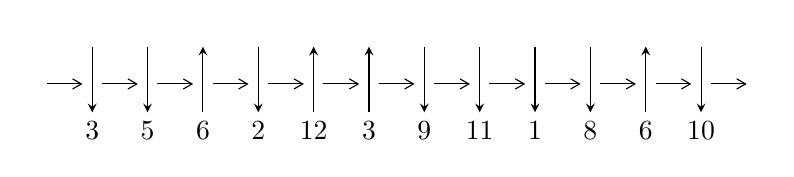
\begin{tikzpicture}[x=20pt, y=17pt]
	% nodes
	\node (C0) at (0, 0) {};
	\node (C1) at (1, 0) {};
	\node (C1U) at (1, +1) {};
	\node (C1D) at (1, -1) {3};

	\node (C2) at (2, 0) {};
	\node (C2U) at (2, +1) {};
	\node (C2D) at (2, -1) {5};

	\node (C3) at (3, 0) {};
	\node (C3U) at (3, +1) {};
	\node (C3D) at (3, -1) {6};

	\node (C4) at (4, 0) {};
	\node (C4U) at (4, +1) {};
	\node (C4D) at (4, -1) {2};

	\node (C5) at (5, 0) {};
	\node (C5U) at (5, +1) {};
	\node (C5D) at (5, -1) {12};

	\node (C6) at (6, 0) {};
	\node (C6U) at (6, +1) {};
	\node (C6D) at (6, -1) {3};

	\node (C7) at (7, 0) {};
	\node (C7U) at (7, +1) {};
	\node (C7D) at (7, -1) {9};

	\node (C8) at (8, 0) {};
	\node (C8U) at (8, +1) {};
	\node (C8D) at (8, -1) {11};

	\node (C9) at (9, 0) {};
	\node (C9U) at (9, +1) {};
	\node (C9D) at (9, -1) {1};

	\node (C10) at (10, 0) {};
	\node (C10U) at (10, +1) {};
	\node (C10D) at (10, -1) {8};

	\node (C11) at (11, 0) {};
	\node (C11U) at (11, +1) {};
	\node (C11D) at (11, -1) {6};

	\node (C12) at (12, 0) {};
	\node (C12U) at (12, +1) {};
	\node (C12D) at (12, -1) {10};
	\node (C13) at (13, 0) {};

	% arrows
	\draw[->,>={angle 60}]
	(C0) edge (C1) (C1) edge (C2) (C2) edge (C3) (C3) edge (C4) (C4) edge (C5) (C5) edge (C6) (C6) edge (C7) (C7) edge (C8) (C8) edge (C9) (C9) edge (C10) (C10) edge (C11) (C11) edge (C12) (C12) edge (C13) ;	\draw[->,>=stealth]
	(C1U) edge (C1D) (C2U) edge (C2D) (C3D) edge (C3U) (C4U) edge (C4D) (C5D) edge (C5U) (C6D) edge (C6U) (C7U) edge (C7D) (C8U) edge (C8D) (C9U) edge (C9D) (C10U) edge (C10D) (C11D) edge (C11U) (C12U) edge (C12D) ;
	\end{tikzpicture} \\
\hhline{~~} \\& 
\textbf{Solving Sequence} \\ \cline{2-2} 
 &
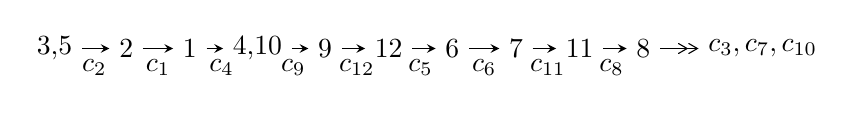
\begin{tikzpicture}[x=23pt, y=7pt]
	% node
	\node (A0) at (-1/8, 0) {3,5};
	\node (A1) at (1, 0) {2};
	\node (A2) at (2, 0) {1};
	\node (A3) at (49/16, 0) {4,10};
	\node (A4) at (33/8, 0) {9};
	\node (A5) at (41/8, 0) {12};
	\node (A6) at (49/8, 0) {6};
	\node (A7) at (57/8, 0) {7};
	\node (A8) at (65/8, 0) {11};
	\node (A9) at (73/8, 0) {8};
	\node (C1) at (1/2, -1) {$c_{2}$};
	\node (C2) at (3/2, -1) {$c_{1}$};
	\node (C3) at (5/2, -1) {$c_{4}$};
	\node (C4) at (29/8, -1) {$c_{9}$};
	\node (C5) at (37/8, -1) {$c_{12}$};
	\node (C6) at (45/8, -1) {$c_{5}$};
	\node (C7) at (53/8, -1) {$c_{6}$};
	\node (C8) at (61/8, -1) {$c_{11}$};
	\node (C9) at (69/8, -1) {$c_{8}$};
	\node (A10) at (11, 0) {$c_{3},c_{7},c_{10}$};

	% edge
	\draw[->,>=stealth]	
	(A0) edge (A1) (A1) edge (A2) (A2) edge (A3) (A3) edge (A4) (A4) edge (A5) (A5) edge (A6) (A6) edge (A7) (A7) edge (A8) (A8) edge (A9) ;
	\draw[->>,>={angle 60}]	
	(A9) edge (A10);
\end{tikzpicture} \\ 

\end{tabular} \\

\footnotetext{
The image of knot diagram is generated by the software ``\textbf{Draw programme}" developed by Andrew Bartholomew(\url{http://www.layer8.co.uk/maths/draw/index.htm\#Running-draw}), where we modified some parts for our purpose(\url{https://github.com/CATsTAILs/LinksPainter}).
}\phantom \\ \newline 
\centering \textbf{Ideals for irreducible components\footnotemark of $X_{\text{par}}$} 
 
\begin{align*}
I^u_{1}&=\langle 
2.86219\times10^{101} u^{65}+3.04230\times10^{102} u^{64}+\cdots+1.07604\times10^{101} b-6.59997\times10^{101},\\
\phantom{I^u_{1}}&\phantom{= \langle  }1.26922\times10^{102} u^{65}+1.35759\times10^{103} u^{64}+\cdots+2.15207\times10^{101} a-2.45951\times10^{103},\\
\phantom{I^u_{1}}&\phantom{= \langle  }u^{66}+11 u^{65}+\cdots-184 u-1\rangle \\
I^u_{2}&=\langle 
-2 a^8+3 a^7-6 a^6+5 a^5-9 a^4+6 a^3-8 a^2+b+3 a-4,\;a^9- a^8+2 a^7- a^6+3 a^5- a^4+2 a^3+a+1,\;u-1\rangle \\
I^u_{3}&=\langle 
u^4+u^3- u^2+b-2 u-1,\;- u^5- u^4+u^3+u^2+a- u-1,\;u^6+u^5- u^4-2 u^3+u+1\rangle \\
\\
\end{align*}
\raggedright * 3 irreducible components of $\dim_{\mathbb{C}}=0$, with total 81 representations.\\
\footnotetext{All coefficients of polynomials are rational numbers. But the coefficients are sometimes approximated in decimal forms when there is not enough margin.}
\newpage
\renewcommand{\arraystretch}{1}
\centering \section*{I. $I^u_{1}= \langle 2.86\times10^{101} u^{65}+3.04\times10^{102} u^{64}+\cdots+1.08\times10^{101} b-6.60\times10^{101},\;1.27\times10^{102} u^{65}+1.36\times10^{103} u^{64}+\cdots+2.15\times10^{101} a-2.46\times10^{103},\;u^{66}+11 u^{65}+\cdots-184 u-1 \rangle$}
\flushleft \textbf{(i) Arc colorings}\\
\begin{tabular}{m{7pt} m{180pt} m{7pt} m{180pt} }
\flushright $a_{3}=$&$\begin{pmatrix}1\\0\end{pmatrix}$ \\
\flushright $a_{5}=$&$\begin{pmatrix}0\\u\end{pmatrix}$ \\
\flushright $a_{2}=$&$\begin{pmatrix}1\\- u^2\end{pmatrix}$ \\
\flushright $a_{1}=$&$\begin{pmatrix}- u^2+1\\- u^2\end{pmatrix}$ \\
\flushright $a_{4}=$&$\begin{pmatrix}u\\- u^3+u\end{pmatrix}$ \\
\flushright $a_{10}=$&$\begin{pmatrix}-5.89768 u^{65}-63.0828 u^{64}+\cdots+2827.10 u+114.286\\-2.65994 u^{65}-28.2732 u^{64}+\cdots+1025.61 u+6.13360\end{pmatrix}$ \\
\flushright $a_{9}=$&$\begin{pmatrix}-8.52453 u^{65}-90.7723 u^{64}+\cdots+3834.57 u+120.324\\-2.57433 u^{65}-27.0269 u^{64}+\cdots+862.488 u+5.23234\end{pmatrix}$ \\
\flushright $a_{12}=$&$\begin{pmatrix}-8.72655 u^{65}-89.2240 u^{64}+\cdots+1798.25 u-38.9602\\-5.28403 u^{65}-54.4051 u^{64}+\cdots+1316.97 u+6.95585\end{pmatrix}$ \\
\flushright $a_{6}=$&$\begin{pmatrix}-3.83893 u^{65}-41.0224 u^{64}+\cdots+1345.05 u-6.03327\\-1.51701 u^{65}-16.1400 u^{64}+\cdots+494.366 u+2.63312\end{pmatrix}$ \\
\flushright $a_{7}=$&$\begin{pmatrix}-5.35594 u^{65}-57.1624 u^{64}+\cdots+1839.41 u-3.40015\\-1.51701 u^{65}-16.1400 u^{64}+\cdots+494.366 u+2.63312\end{pmatrix}$ \\
\flushright $a_{11}=$&$\begin{pmatrix}13.7708 u^{65}+144.182 u^{64}+\cdots-4481.24 u-77.0429\\0.429501 u^{65}+4.69148 u^{64}+\cdots-219.153 u-1.47738\end{pmatrix}$ \\
\flushright $a_{8}=$&$\begin{pmatrix}-7.65340 u^{65}-81.3957 u^{64}+\cdots+3054.18 u+72.2685\\-5.10197 u^{65}-53.2822 u^{64}+\cdots+1553.54 u+8.78813\end{pmatrix}$\\&\end{tabular}
\flushleft \textbf{(ii) Obstruction class $= -1$}\\~\\
\flushleft \textbf{(iii) Cusp Shapes $= 7.00145 u^{65}+70.4042 u^{64}+\cdots-636.383 u-12.3310$}\\~\\
\newpage\renewcommand{\arraystretch}{1}
\flushleft \textbf{(iv) u-Polynomials at the component}\newline \\
\begin{tabular}{m{50pt}|m{274pt}}
Crossings & \hspace{64pt}u-Polynomials at each crossing \\
\hline $$\begin{aligned}c_{1}\end{aligned}$$&$\begin{aligned}
&u^{66}+21 u^{65}+\cdots+31524 u+1
\end{aligned}$\\
\hline $$\begin{aligned}c_{2},c_{4}\end{aligned}$$&$\begin{aligned}
&u^{66}-11 u^{65}+\cdots+184 u-1
\end{aligned}$\\
\hline $$\begin{aligned}c_{3},c_{6}\end{aligned}$$&$\begin{aligned}
&u^{66}+8 u^{65}+\cdots-7168 u+512
\end{aligned}$\\
\hline $$\begin{aligned}c_{5},c_{11}\end{aligned}$$&$\begin{aligned}
&u^{66}+3 u^{65}+\cdots-2 u-1
\end{aligned}$\\
\hline $$\begin{aligned}c_{7}\end{aligned}$$&$\begin{aligned}
&u^{66}+28 u^{65}+\cdots-143 u+1
\end{aligned}$\\
\hline $$\begin{aligned}c_{8},c_{10}\end{aligned}$$&$\begin{aligned}
&u^{66}-8 u^{65}+\cdots-11 u+1
\end{aligned}$\\
\hline $$\begin{aligned}c_{9},c_{12}\end{aligned}$$&$\begin{aligned}
&u^{66}-2 u^{65}+\cdots+192 u+64
\end{aligned}$\\
\hline
\end{tabular}\\~\\
\newpage\renewcommand{\arraystretch}{1}
\flushleft \textbf{(v) Riley Polynomials at the component}\newline \\
\begin{tabular}{m{50pt}|m{274pt}}
Crossings & \hspace{64pt}Riley Polynomials at each crossing \\
\hline $$\begin{aligned}c_{1}\end{aligned}$$&$\begin{aligned}
&y^{66}+59 y^{65}+\cdots-992297680 y+1
\end{aligned}$\\
\hline $$\begin{aligned}c_{2},c_{4}\end{aligned}$$&$\begin{aligned}
&y^{66}-21 y^{65}+\cdots-31524 y+1
\end{aligned}$\\
\hline $$\begin{aligned}c_{3},c_{6}\end{aligned}$$&$\begin{aligned}
&y^{66}-60 y^{65}+\cdots-76021760 y+262144
\end{aligned}$\\
\hline $$\begin{aligned}c_{5},c_{11}\end{aligned}$$&$\begin{aligned}
&y^{66}+15 y^{65}+\cdots-20 y+1
\end{aligned}$\\
\hline $$\begin{aligned}c_{7}\end{aligned}$$&$\begin{aligned}
&y^{66}+28 y^{65}+\cdots-12229 y+1
\end{aligned}$\\
\hline $$\begin{aligned}c_{8},c_{10}\end{aligned}$$&$\begin{aligned}
&y^{66}-28 y^{65}+\cdots+143 y+1
\end{aligned}$\\
\hline $$\begin{aligned}c_{9},c_{12}\end{aligned}$$&$\begin{aligned}
&y^{66}+42 y^{65}+\cdots+77824 y+4096
\end{aligned}$\\
\hline
\end{tabular}\\~\\
\newpage\flushleft \textbf{(vi) Complex Volumes and Cusp Shapes}
$$\begin{array}{c|c|c}  
\text{Solutions to }I^u_{1}& \I (\text{vol} + \sqrt{-1}CS) & \text{Cusp shape}\\
 \hline 
\begin{aligned}
u &= \phantom{-}1.00537\phantom{ +0.000000I} \\
a &= \phantom{-}0.406767\phantom{ +0.000000I} \\
b &= -11.0855\phantom{ +0.000000I}\end{aligned}
 & -2.82917\phantom{ +0.000000I} & \phantom{-}365.350\phantom{ +0.000000I} \\ \hline\begin{aligned}
u &= \phantom{-}0.687723 + 0.687263 I \\
a &= -1.353200 - 0.228510 I \\
b &= -1.300520 + 0.290425 I\end{aligned}
 & -2.23471 - 2.98196 I & \phantom{-0.000000 } 0 \\ \hline\begin{aligned}
u &= \phantom{-}0.687723 - 0.687263 I \\
a &= -1.353200 + 0.228510 I \\
b &= -1.300520 - 0.290425 I\end{aligned}
 & -2.23471 + 2.98196 I & \phantom{-0.000000 } 0 \\ \hline\begin{aligned}
u &= \phantom{-}1.028820 + 0.216167 I \\
a &= \phantom{-}0.012733 + 0.445672 I \\
b &= \phantom{-}0.438763 + 0.902849 I\end{aligned}
 & -1.91057 - 0.79816 I & \phantom{-0.000000 } 0 \\ \hline\begin{aligned}
u &= \phantom{-}1.028820 - 0.216167 I \\
a &= \phantom{-}0.012733 - 0.445672 I \\
b &= \phantom{-}0.438763 - 0.902849 I\end{aligned}
 & -1.91057 + 0.79816 I & \phantom{-0.000000 } 0 \\ \hline\begin{aligned}
u &= \phantom{-}0.783333 + 0.429567 I \\
a &= \phantom{-}2.12816 + 1.63033 I \\
b &= \phantom{-}2.36643 - 1.94607 I\end{aligned}
 & -3.21013 - 1.26950 I & -4.00000 + 7.64083 I \\ \hline\begin{aligned}
u &= \phantom{-}0.783333 - 0.429567 I \\
a &= \phantom{-}2.12816 - 1.63033 I \\
b &= \phantom{-}2.36643 + 1.94607 I\end{aligned}
 & -3.21013 + 1.26950 I & -4.00000 - 7.64083 I \\ \hline\begin{aligned}
u &= \phantom{-}1.125970 + 0.056995 I \\
a &= \phantom{-}0.023922 - 0.599547 I \\
b &= \phantom{-}0.36398 + 1.57344 I\end{aligned}
 & \phantom{-}0.81136 + 2.64313 I & \phantom{-0.000000 } 0 \\ \hline\begin{aligned}
u &= \phantom{-}1.125970 - 0.056995 I \\
a &= \phantom{-}0.023922 + 0.599547 I \\
b &= \phantom{-}0.36398 - 1.57344 I\end{aligned}
 & \phantom{-}0.81136 - 2.64313 I & \phantom{-0.000000 } 0 \\ \hline\begin{aligned}
u &= -0.824004 + 0.171548 I \\
a &= -1.143160 + 0.689270 I \\
b &= -0.151706 + 0.583718 I\end{aligned}
 & -4.86194 + 7.45999 I & -0.96246 - 11.41011 I\\
 \hline 
 \end{array}$$\newpage$$\begin{array}{c|c|c}  
\text{Solutions to }I^u_{1}& \I (\text{vol} + \sqrt{-1}CS) & \text{Cusp shape}\\
 \hline 
\begin{aligned}
u &= -0.824004 - 0.171548 I \\
a &= -1.143160 - 0.689270 I \\
b &= -0.151706 - 0.583718 I\end{aligned}
 & -4.86194 - 7.45999 I & -0.96246 + 11.41011 I \\ \hline\begin{aligned}
u &= \phantom{-}0.515278 + 1.048940 I \\
a &= -1.36638 - 1.36297 I \\
b &= -1.375720 + 0.022642 I\end{aligned}
 & \phantom{-}2.19847 - 2.32521 I & \phantom{-0.000000 } 0 \\ \hline\begin{aligned}
u &= \phantom{-}0.515278 - 1.048940 I \\
a &= -1.36638 + 1.36297 I \\
b &= -1.375720 - 0.022642 I\end{aligned}
 & \phantom{-}2.19847 + 2.32521 I & \phantom{-0.000000 } 0 \\ \hline\begin{aligned}
u &= -0.745847 + 0.910266 I \\
a &= -1.20178 + 2.28035 I \\
b &= -2.03130 + 0.52431 I\end{aligned}
 & \phantom{-}2.17496 - 0.19887 I & \phantom{-0.000000 } 0 \\ \hline\begin{aligned}
u &= -0.745847 - 0.910266 I \\
a &= -1.20178 - 2.28035 I \\
b &= -2.03130 - 0.52431 I\end{aligned}
 & \phantom{-}2.17496 + 0.19887 I & \phantom{-0.000000 } 0 \\ \hline\begin{aligned}
u &= -0.760288 + 0.928501 I \\
a &= \phantom{-}1.67368 - 0.06126 I \\
b &= \phantom{-}1.88450 + 0.90427 I\end{aligned}
 & \phantom{-}7.72304 - 2.79945 I & \phantom{-0.000000 } 0 \\ \hline\begin{aligned}
u &= -0.760288 - 0.928501 I \\
a &= \phantom{-}1.67368 + 0.06126 I \\
b &= \phantom{-}1.88450 - 0.90427 I\end{aligned}
 & \phantom{-}7.72304 + 2.79945 I & \phantom{-0.000000 } 0 \\ \hline\begin{aligned}
u &= \phantom{-}0.668448 + 0.397576 I \\
a &= \phantom{-}0.003744 - 1.234270 I \\
b &= -1.38255 + 1.28759 I\end{aligned}
 & \phantom{-}2.07274 - 4.10478 I & -2.27198 - 0.09641 I \\ \hline\begin{aligned}
u &= \phantom{-}0.668448 - 0.397576 I \\
a &= \phantom{-}0.003744 + 1.234270 I \\
b &= -1.38255 - 1.28759 I\end{aligned}
 & \phantom{-}2.07274 + 4.10478 I & -2.27198 + 0.09641 I \\ \hline\begin{aligned}
u &= -0.856203 + 0.882898 I \\
a &= \phantom{-}0.290557 + 1.073450 I \\
b &= \phantom{-}0.231042 + 0.438928 I\end{aligned}
 & \phantom{-}3.57906 + 2.47635 I & \phantom{-0.000000 } 0\\
 \hline 
 \end{array}$$\newpage$$\begin{array}{c|c|c}  
\text{Solutions to }I^u_{1}& \I (\text{vol} + \sqrt{-1}CS) & \text{Cusp shape}\\
 \hline 
\begin{aligned}
u &= -0.856203 - 0.882898 I \\
a &= \phantom{-}0.290557 - 1.073450 I \\
b &= \phantom{-}0.231042 - 0.438928 I\end{aligned}
 & \phantom{-}3.57906 - 2.47635 I & \phantom{-0.000000 } 0 \\ \hline\begin{aligned}
u &= -1.118290 + 0.517016 I \\
a &= \phantom{-}0.122393 - 0.353509 I \\
b &= -0.055274 - 0.183449 I\end{aligned}
 & -1.20228 + 5.48361 I & \phantom{-0.000000 } 0 \\ \hline\begin{aligned}
u &= -1.118290 - 0.517016 I \\
a &= \phantom{-}0.122393 + 0.353509 I \\
b &= -0.055274 + 0.183449 I\end{aligned}
 & -1.20228 - 5.48361 I & \phantom{-0.000000 } 0 \\ \hline\begin{aligned}
u &= -0.690354 + 1.028160 I \\
a &= -0.438411 - 1.018090 I \\
b &= -0.341152 - 0.391855 I\end{aligned}
 & \phantom{-}4.03833 - 2.66127 I & \phantom{-0.000000 } 0 \\ \hline\begin{aligned}
u &= -0.690354 - 1.028160 I \\
a &= -0.438411 + 1.018090 I \\
b &= -0.341152 + 0.391855 I\end{aligned}
 & \phantom{-}4.03833 + 2.66127 I & \phantom{-0.000000 } 0 \\ \hline\begin{aligned}
u &= \phantom{-}1.274370 + 0.103527 I \\
a &= \phantom{-}0.09874 + 1.51084 I \\
b &= \phantom{-}1.63942 + 2.71558 I\end{aligned}
 & -4.31795 - 0.78820 I & \phantom{-0.000000 } 0 \\ \hline\begin{aligned}
u &= \phantom{-}1.274370 - 0.103527 I \\
a &= \phantom{-}0.09874 - 1.51084 I \\
b &= \phantom{-}1.63942 - 2.71558 I\end{aligned}
 & -4.31795 + 0.78820 I & \phantom{-0.000000 } 0 \\ \hline\begin{aligned}
u &= -0.983683 + 0.830782 I \\
a &= \phantom{-}0.570504 + 0.494511 I \\
b &= \phantom{-}0.437347 + 0.006156 I\end{aligned}
 & \phantom{-}3.17239 + 3.89822 I & \phantom{-0.000000 } 0 \\ \hline\begin{aligned}
u &= -0.983683 - 0.830782 I \\
a &= \phantom{-}0.570504 - 0.494511 I \\
b &= \phantom{-}0.437347 - 0.006156 I\end{aligned}
 & \phantom{-}3.17239 - 3.89822 I & \phantom{-0.000000 } 0 \\ \hline\begin{aligned}
u &= -0.894353 + 0.951169 I \\
a &= -1.78516 + 0.28107 I \\
b &= -2.14588 - 0.82546 I\end{aligned}
 & \phantom{-}9.29382 + 3.78649 I & \phantom{-0.000000 } 0\\
 \hline 
 \end{array}$$\newpage$$\begin{array}{c|c|c}  
\text{Solutions to }I^u_{1}& \I (\text{vol} + \sqrt{-1}CS) & \text{Cusp shape}\\
 \hline 
\begin{aligned}
u &= -0.894353 - 0.951169 I \\
a &= -1.78516 - 0.28107 I \\
b &= -2.14588 + 0.82546 I\end{aligned}
 & \phantom{-}9.29382 - 3.78649 I & \phantom{-0.000000 } 0 \\ \hline\begin{aligned}
u &= -1.062290 + 0.802217 I \\
a &= \phantom{-}2.22217 - 0.70557 I \\
b &= \phantom{-}2.85845 + 0.87099 I\end{aligned}
 & \phantom{-}1.18870 + 6.56344 I & \phantom{-0.000000 } 0 \\ \hline\begin{aligned}
u &= -1.062290 - 0.802217 I \\
a &= \phantom{-}2.22217 + 0.70557 I \\
b &= \phantom{-}2.85845 - 0.87099 I\end{aligned}
 & \phantom{-}1.18870 - 6.56344 I & \phantom{-0.000000 } 0 \\ \hline\begin{aligned}
u &= -1.057290 + 0.809211 I \\
a &= -0.51219 + 1.44953 I \\
b &= -1.79007 + 0.34040 I\end{aligned}
 & \phantom{-}6.78475 + 9.23321 I & \phantom{-0.000000 } 0 \\ \hline\begin{aligned}
u &= -1.057290 - 0.809211 I \\
a &= -0.51219 - 1.44953 I \\
b &= -1.79007 - 0.34040 I\end{aligned}
 & \phantom{-}6.78475 - 9.23321 I & \phantom{-0.000000 } 0 \\ \hline\begin{aligned}
u &= -0.620743 + 0.209791 I \\
a &= \phantom{-}1.51472 - 0.44133 I \\
b &= \phantom{-}0.351541 - 0.610430 I\end{aligned}
 & -1.43375 + 2.91518 I & \phantom{-}0.46506 - 4.85019 I \\ \hline\begin{aligned}
u &= -0.620743 - 0.209791 I \\
a &= \phantom{-}1.51472 + 0.44133 I \\
b &= \phantom{-}0.351541 + 0.610430 I\end{aligned}
 & -1.43375 - 2.91518 I & \phantom{-}0.46506 + 4.85019 I \\ \hline\begin{aligned}
u &= -0.597235 + 0.259408 I \\
a &= -0.28543 + 1.39421 I \\
b &= -0.011224 + 0.406559 I\end{aligned}
 & \phantom{-}1.17931 - 1.63015 I & \phantom{-}3.12613 + 3.30141 I \\ \hline\begin{aligned}
u &= -0.597235 - 0.259408 I \\
a &= -0.28543 - 1.39421 I \\
b &= -0.011224 - 0.406559 I\end{aligned}
 & \phantom{-}1.17931 + 1.63015 I & \phantom{-}3.12613 - 3.30141 I \\ \hline\begin{aligned}
u &= -0.994697 + 0.913978 I \\
a &= \phantom{-}0.79592 - 1.57410 I \\
b &= \phantom{-}1.87674 - 0.36992 I\end{aligned}
 & \phantom{-}8.98485 + 3.05406 I & \phantom{-0.000000 } 0\\
 \hline 
 \end{array}$$\newpage$$\begin{array}{c|c|c}  
\text{Solutions to }I^u_{1}& \I (\text{vol} + \sqrt{-1}CS) & \text{Cusp shape}\\
 \hline 
\begin{aligned}
u &= -0.994697 - 0.913978 I \\
a &= \phantom{-}0.79592 + 1.57410 I \\
b &= \phantom{-}1.87674 + 0.36992 I\end{aligned}
 & \phantom{-}8.98485 - 3.05406 I & \phantom{-0.000000 } 0 \\ \hline\begin{aligned}
u &= \phantom{-}0.784334 + 1.103720 I \\
a &= \phantom{-}1.32414 + 1.54204 I \\
b &= \phantom{-}1.68117 + 0.18497 I\end{aligned}
 & \phantom{-}1.02644 - 7.74901 I & \phantom{-0.000000 } 0 \\ \hline\begin{aligned}
u &= \phantom{-}0.784334 - 1.103720 I \\
a &= \phantom{-}1.32414 - 1.54204 I \\
b &= \phantom{-}1.68117 - 0.18497 I\end{aligned}
 & \phantom{-}1.02644 + 7.74901 I & \phantom{-0.000000 } 0 \\ \hline\begin{aligned}
u &= -0.634943 + 0.050863 I \\
a &= -1.58118 - 0.94089 I \\
b &= -0.349515 - 0.878817 I\end{aligned}
 & -5.23148 + 1.44469 I & -2.19147 - 1.36304 I \\ \hline\begin{aligned}
u &= -0.634943 - 0.050863 I \\
a &= -1.58118 + 0.94089 I \\
b &= -0.349515 + 0.878817 I\end{aligned}
 & -5.23148 - 1.44469 I & -2.19147 + 1.36304 I \\ \hline\begin{aligned}
u &= \phantom{-}0.601289 + 0.105594 I \\
a &= \phantom{-}0.258323 + 0.970497 I \\
b &= \phantom{-}1.215100 - 0.178401 I\end{aligned}
 & -1.82059 + 0.01526 I & -7.87182 - 0.48568 I \\ \hline\begin{aligned}
u &= \phantom{-}0.601289 - 0.105594 I \\
a &= \phantom{-}0.258323 - 0.970497 I \\
b &= \phantom{-}1.215100 + 0.178401 I\end{aligned}
 & -1.82059 - 0.01526 I & -7.87182 + 0.48568 I \\ \hline\begin{aligned}
u &= -1.127320 + 0.826259 I \\
a &= -0.431491 - 0.571092 I \\
b &= -0.399530 - 0.114576 I\end{aligned}
 & \phantom{-}2.66554 + 9.42263 I & \phantom{-0.000000 } 0 \\ \hline\begin{aligned}
u &= -1.127320 - 0.826259 I \\
a &= -0.431491 + 0.571092 I \\
b &= -0.399530 + 0.114576 I\end{aligned}
 & \phantom{-}2.66554 - 9.42263 I & \phantom{-0.000000 } 0 \\ \hline\begin{aligned}
u &= -0.147109 + 0.577451 I \\
a &= -1.41532 - 0.01491 I \\
b &= -0.366040 + 0.326712 I\end{aligned}
 & \phantom{-}1.31523 - 1.27199 I & \phantom{-}3.06090 + 2.68907 I\\
 \hline 
 \end{array}$$\newpage$$\begin{array}{c|c|c}  
\text{Solutions to }I^u_{1}& \I (\text{vol} + \sqrt{-1}CS) & \text{Cusp shape}\\
 \hline 
\begin{aligned}
u &= -0.147109 - 0.577451 I \\
a &= -1.41532 + 0.01491 I \\
b &= -0.366040 - 0.326712 I\end{aligned}
 & \phantom{-}1.31523 + 1.27199 I & \phantom{-}3.06090 - 2.68907 I \\ \hline\begin{aligned}
u &= -0.723739 + 1.209940 I \\
a &= \phantom{-}1.67771 - 1.53567 I \\
b &= \phantom{-}2.06140 - 0.32997 I\end{aligned}
 & \phantom{-}9.83371 - 2.67210 I & \phantom{-0.000000 } 0 \\ \hline\begin{aligned}
u &= -0.723739 - 1.209940 I \\
a &= \phantom{-}1.67771 + 1.53567 I \\
b &= \phantom{-}2.06140 + 0.32997 I\end{aligned}
 & \phantom{-}9.83371 + 2.67210 I & \phantom{-0.000000 } 0 \\ \hline\begin{aligned}
u &= \phantom{-}0.411231 + 0.411306 I \\
a &= \phantom{-}0.32779 + 1.74947 I \\
b &= \phantom{-}0.97919 - 1.06319 I\end{aligned}
 & \phantom{-}2.74552 + 1.51786 I & -0.89722 - 4.70084 I \\ \hline\begin{aligned}
u &= \phantom{-}0.411231 - 0.411306 I \\
a &= \phantom{-}0.32779 - 1.74947 I \\
b &= \phantom{-}0.97919 + 1.06319 I\end{aligned}
 & \phantom{-}2.74552 - 1.51786 I & -0.89722 + 4.70084 I \\ \hline\begin{aligned}
u &= -0.60092 + 1.28586 I \\
a &= -1.89989 + 1.40726 I \\
b &= -2.07450 + 0.29742 I\end{aligned}
 & \phantom{-}8.19227 - 8.99833 I & \phantom{-0.000000 } 0 \\ \hline\begin{aligned}
u &= -0.60092 - 1.28586 I \\
a &= -1.89989 - 1.40726 I \\
b &= -2.07450 - 0.29742 I\end{aligned}
 & \phantom{-}8.19227 + 8.99833 I & \phantom{-0.000000 } 0 \\ \hline\begin{aligned}
u &= -1.19778 + 0.88601 I \\
a &= -1.78025 + 0.89840 I \\
b &= -2.69078 - 0.32973 I\end{aligned}
 & \phantom{-}8.24876 + 10.14770 I & \phantom{-0.000000 } 0 \\ \hline\begin{aligned}
u &= -1.19778 - 0.88601 I \\
a &= -1.78025 - 0.89840 I \\
b &= -2.69078 + 0.32973 I\end{aligned}
 & \phantom{-}8.24876 - 10.14770 I & \phantom{-0.000000 } 0 \\ \hline\begin{aligned}
u &= -1.26526 + 0.84227 I \\
a &= \phantom{-}1.68547 - 1.04922 I \\
b &= \phantom{-}2.75955 + 0.13511 I\end{aligned}
 & \phantom{-}5.9981 + 16.5072 I & \phantom{-0.000000 } 0\\
 \hline 
 \end{array}$$\newpage$$\begin{array}{c|c|c}  
\text{Solutions to }I^u_{1}& \I (\text{vol} + \sqrt{-1}CS) & \text{Cusp shape}\\
 \hline 
\begin{aligned}
u &= -1.26526 - 0.84227 I \\
a &= \phantom{-}1.68547 + 1.04922 I \\
b &= \phantom{-}2.75955 - 0.13511 I\end{aligned}
 & \phantom{-}5.9981 - 16.5072 I & \phantom{-0.000000 } 0 \\ \hline\begin{aligned}
u &= \phantom{-}1.42330 + 0.57117 I \\
a &= -0.920325 + 0.724904 I \\
b &= -1.27403 + 1.04616 I\end{aligned}
 & -1.42259 + 0.46359 I & \phantom{-0.000000 } 0 \\ \hline\begin{aligned}
u &= \phantom{-}1.42330 - 0.57117 I \\
a &= -0.920325 - 0.724904 I \\
b &= -1.27403 - 1.04616 I\end{aligned}
 & -1.42259 - 0.46359 I & \phantom{-0.000000 } 0 \\ \hline\begin{aligned}
u &= \phantom{-}1.59839 + 0.34758 I \\
a &= \phantom{-}0.832676 - 0.993612 I \\
b &= \phantom{-}1.38737 - 1.32476 I\end{aligned}
 & -1.87995 - 4.31692 I & \phantom{-0.000000 } 0 \\ \hline\begin{aligned}
u &= \phantom{-}1.59839 - 0.34758 I \\
a &= \phantom{-}0.832676 + 0.993612 I \\
b &= \phantom{-}1.38737 + 1.32476 I\end{aligned}
 & -1.87995 + 4.31692 I & \phantom{-0.000000 } 0 \\ \hline\begin{aligned}
u &= -0.00563429\phantom{ +0.000000I} \\
a &= \phantom{-}98.6949\phantom{ +0.000000I} \\
b &= \phantom{-}0.501097\phantom{ +0.000000I}\end{aligned}
 & -1.20362\phantom{ +0.000000I} & -8.91660\phantom{ +0.000000I}\\
 \hline 
 \end{array}$$\newpage\newpage\renewcommand{\arraystretch}{1}
\centering \section*{II. $I^u_{2}= \langle -2 a^8+b+\cdots+3 a-4,\;a^9- a^8+2 a^7- a^6+3 a^5- a^4+2 a^3+a+1,\;u-1 \rangle$}
\flushleft \textbf{(i) Arc colorings}\\
\begin{tabular}{m{7pt} m{180pt} m{7pt} m{180pt} }
\flushright $a_{3}=$&$\begin{pmatrix}1\\0\end{pmatrix}$ \\
\flushright $a_{5}=$&$\begin{pmatrix}0\\1\end{pmatrix}$ \\
\flushright $a_{2}=$&$\begin{pmatrix}1\\-1\end{pmatrix}$ \\
\flushright $a_{1}=$&$\begin{pmatrix}0\\-1\end{pmatrix}$ \\
\flushright $a_{4}=$&$\begin{pmatrix}1\\0\end{pmatrix}$ \\
\flushright $a_{10}=$&$\begin{pmatrix}a\\2 a^8-3 a^7+6 a^6-5 a^5+9 a^4-6 a^3+8 a^2-3 a+4\end{pmatrix}$ \\
\flushright $a_{9}=$&$\begin{pmatrix}a\\2 a^8-3 a^7+6 a^6-5 a^5+9 a^4-6 a^3+8 a^2-4 a+4\end{pmatrix}$ \\
\flushright $a_{12}=$&$\begin{pmatrix}- a^2\\a^8-2 a^7+3 a^6-3 a^5+4 a^4-4 a^3+3 a^2-2 a+1\end{pmatrix}$ \\
\flushright $a_{6}=$&$\begin{pmatrix}a^4\\0\end{pmatrix}$ \\
\flushright $a_{7}=$&$\begin{pmatrix}a^4\\0\end{pmatrix}$ \\
\flushright $a_{11}=$&$\begin{pmatrix}- a^6- a^2\\a^8-2 a^7+3 a^6-3 a^5+4 a^4-4 a^3+3 a^2-2 a+1\end{pmatrix}$ \\
\flushright $a_{8}=$&$\begin{pmatrix}- a^6- a^2\\a^8-2 a^7+4 a^6-3 a^5+6 a^4-4 a^3+6 a^2-2 a+3\end{pmatrix}$\\&\end{tabular}
\flushleft \textbf{(ii) Obstruction class $= 1$}\\~\\
\flushleft \textbf{(iii) Cusp Shapes $= -45 a^8+71 a^7-127 a^6+112 a^5-192 a^4+149 a^3-165 a^2+83 a-97$}\\~\\
\newpage\renewcommand{\arraystretch}{1}
\flushleft \textbf{(iv) u-Polynomials at the component}\newline \\
\begin{tabular}{m{50pt}|m{274pt}}
Crossings & \hspace{64pt}u-Polynomials at each crossing \\
\hline $$\begin{aligned}c_{1},c_{2}\end{aligned}$$&$\begin{aligned}
&(u-1)^9
\end{aligned}$\\
\hline $$\begin{aligned}c_{3},c_{6}\end{aligned}$$&$\begin{aligned}
&u^9
\end{aligned}$\\
\hline $$\begin{aligned}c_{4}\end{aligned}$$&$\begin{aligned}
&(u+1)^9
\end{aligned}$\\
\hline $$\begin{aligned}c_{5}\end{aligned}$$&$\begin{aligned}
&u^9+3 u^8+8 u^7+13 u^6+17 u^5+17 u^4+12 u^3+6 u^2+u-1
\end{aligned}$\\
\hline $$\begin{aligned}c_{7}\end{aligned}$$&$\begin{aligned}
&u^9-5 u^8+12 u^7-15 u^6+9 u^5+u^4-4 u^3+2 u^2+u-1
\end{aligned}$\\
\hline $$\begin{aligned}c_{8}\end{aligned}$$&$\begin{aligned}
&u^9+u^8-2 u^7-3 u^6+u^5+3 u^4+2 u^3- u-1
\end{aligned}$\\
\hline $$\begin{aligned}c_{9}\end{aligned}$$&$\begin{aligned}
&u^9+u^8+2 u^7+u^6+3 u^5+u^4+2 u^3+u-1
\end{aligned}$\\
\hline $$\begin{aligned}c_{10}\end{aligned}$$&$\begin{aligned}
&u^9- u^8-2 u^7+3 u^6+u^5-3 u^4+2 u^3- u+1
\end{aligned}$\\
\hline $$\begin{aligned}c_{11}\end{aligned}$$&$\begin{aligned}
&u^9-3 u^8+8 u^7-13 u^6+17 u^5-17 u^4+12 u^3-6 u^2+u+1
\end{aligned}$\\
\hline $$\begin{aligned}c_{12}\end{aligned}$$&$\begin{aligned}
&u^9- u^8+2 u^7- u^6+3 u^5- u^4+2 u^3+u+1
\end{aligned}$\\
\hline
\end{tabular}\\~\\
\newpage\renewcommand{\arraystretch}{1}
\flushleft \textbf{(v) Riley Polynomials at the component}\newline \\
\begin{tabular}{m{50pt}|m{274pt}}
Crossings & \hspace{64pt}Riley Polynomials at each crossing \\
\hline $$\begin{aligned}c_{1},c_{2},c_{4}\end{aligned}$$&$\begin{aligned}
&(y-1)^9
\end{aligned}$\\
\hline $$\begin{aligned}c_{3},c_{6}\end{aligned}$$&$\begin{aligned}
&y^9
\end{aligned}$\\
\hline $$\begin{aligned}c_{5},c_{11}\end{aligned}$$&$\begin{aligned}
&y^9+7 y^8+20 y^7+25 y^6+5 y^5-15 y^4+22 y^2+13 y-1
\end{aligned}$\\
\hline $$\begin{aligned}c_{7}\end{aligned}$$&$\begin{aligned}
&y^9- y^8+12 y^7-7 y^6+37 y^5+y^4-10 y^2+5 y-1
\end{aligned}$\\
\hline $$\begin{aligned}c_{8},c_{10}\end{aligned}$$&$\begin{aligned}
&y^9-5 y^8+12 y^7-15 y^6+9 y^5+y^4-4 y^3+2 y^2+y-1
\end{aligned}$\\
\hline $$\begin{aligned}c_{9},c_{12}\end{aligned}$$&$\begin{aligned}
&y^9+3 y^8+8 y^7+13 y^6+17 y^5+17 y^4+12 y^3+6 y^2+y-1
\end{aligned}$\\
\hline
\end{tabular}\\~\\
\newpage\flushleft \textbf{(vi) Complex Volumes and Cusp Shapes}
$$\begin{array}{c|c|c}  
\text{Solutions to }I^u_{2}& \I (\text{vol} + \sqrt{-1}CS) & \text{Cusp shape}\\
 \hline 
\begin{aligned}
u &= \phantom{-}1.00000\phantom{ +0.000000I} \\
a &= -0.140343 + 0.966856 I \\
b &= -0.302374 + 0.039314 I\end{aligned}
 & \phantom{-}0.13850 + 2.09337 I & -4.31028 - 3.82038 I \\ \hline\begin{aligned}
u &= \phantom{-}1.00000\phantom{ +0.000000I} \\
a &= -0.140343 - 0.966856 I \\
b &= -0.302374 - 0.039314 I\end{aligned}
 & \phantom{-}0.13850 - 2.09337 I & -4.31028 + 3.82038 I \\ \hline\begin{aligned}
u &= \phantom{-}1.00000\phantom{ +0.000000I} \\
a &= -0.628449 + 0.875112 I \\
b &= -0.223063 + 0.988364 I\end{aligned}
 & -2.26187 + 2.45442 I & -6.95900 - 1.69416 I \\ \hline\begin{aligned}
u &= \phantom{-}1.00000\phantom{ +0.000000I} \\
a &= -0.628449 - 0.875112 I \\
b &= -0.223063 - 0.988364 I\end{aligned}
 & -2.26187 - 2.45442 I & -6.95900 + 1.69416 I \\ \hline\begin{aligned}
u &= \phantom{-}1.00000\phantom{ +0.000000I} \\
a &= \phantom{-}0.796005 + 0.733148 I \\
b &= -0.194585 + 1.248300 I\end{aligned}
 & -6.01628 + 1.33617 I & -13.56769 - 0.26615 I \\ \hline\begin{aligned}
u &= \phantom{-}1.00000\phantom{ +0.000000I} \\
a &= \phantom{-}0.796005 - 0.733148 I \\
b &= -0.194585 - 1.248300 I\end{aligned}
 & -6.01628 - 1.33617 I & -13.56769 + 0.26615 I \\ \hline\begin{aligned}
u &= \phantom{-}1.00000\phantom{ +0.000000I} \\
a &= \phantom{-}0.728966 + 0.986295 I \\
b &= \phantom{-}0.026651 + 0.835796 I\end{aligned}
 & -5.24306 - 7.08493 I & -11.54551 + 1.34000 I \\ \hline\begin{aligned}
u &= \phantom{-}1.00000\phantom{ +0.000000I} \\
a &= \phantom{-}0.728966 - 0.986295 I \\
b &= \phantom{-}0.026651 - 0.835796 I\end{aligned}
 & -5.24306 + 7.08493 I & -11.54551 - 1.34000 I \\ \hline\begin{aligned}
u &= \phantom{-}1.00000\phantom{ +0.000000I} \\
a &= -0.512358\phantom{ +0.000000I} \\
b &= \phantom{-}9.38674\phantom{ +0.000000I}\end{aligned}
 & -2.84338\phantom{ +0.000000I} & -223.240\phantom{ +0.000000I}\\
 \hline 
 \end{array}$$\newpage\newpage\renewcommand{\arraystretch}{1}
\centering \section*{III. $I^u_{3}= \langle u^4+u^3- u^2+b-2 u-1,\;- u^5- u^4+u^3+u^2+a- u-1,\;u^6+u^5- u^4-2 u^3+u+1 \rangle$}
\flushleft \textbf{(i) Arc colorings}\\
\begin{tabular}{m{7pt} m{180pt} m{7pt} m{180pt} }
\flushright $a_{3}=$&$\begin{pmatrix}1\\0\end{pmatrix}$ \\
\flushright $a_{5}=$&$\begin{pmatrix}0\\u\end{pmatrix}$ \\
\flushright $a_{2}=$&$\begin{pmatrix}1\\- u^2\end{pmatrix}$ \\
\flushright $a_{1}=$&$\begin{pmatrix}- u^2+1\\- u^2\end{pmatrix}$ \\
\flushright $a_{4}=$&$\begin{pmatrix}u\\- u^3+u\end{pmatrix}$ \\
\flushright $a_{10}=$&$\begin{pmatrix}u^5+u^4- u^3- u^2+u+1\\- u^4- u^3+u^2+2 u+1\end{pmatrix}$ \\
\flushright $a_{9}=$&$\begin{pmatrix}u^5+u^4- u^3- u^2+u+1\\- u^4- u^3+u^2+2 u+1\end{pmatrix}$ \\
\flushright $a_{12}=$&$\begin{pmatrix}- u^2+1\\- u^2\end{pmatrix}$ \\
\flushright $a_{6}=$&$\begin{pmatrix}u^5-2 u^3+u\\u^5- u^3+u\end{pmatrix}$ \\
\flushright $a_{7}=$&$\begin{pmatrix}2 u^5-3 u^3+2 u\\u^5- u^3+u\end{pmatrix}$ \\
\flushright $a_{11}=$&$\begin{pmatrix}-2 u^5+3 u^3-2 u\\- u^5+u^3- u\end{pmatrix}$ \\
\flushright $a_{8}=$&$\begin{pmatrix}3 u^5+u^4-4 u^3- u^2+3 u+1\\u^5- u^4-2 u^3+u^2+3 u+1\end{pmatrix}$\\&\end{tabular}
\flushleft \textbf{(ii) Obstruction class $= 1$}\\~\\
\flushleft \textbf{(iii) Cusp Shapes $= -3 u^5+u^4- u^3-2 u^2-3 u-7$}\\~\\
\newpage\renewcommand{\arraystretch}{1}
\flushleft \textbf{(iv) u-Polynomials at the component}\newline \\
\begin{tabular}{m{50pt}|m{274pt}}
Crossings & \hspace{64pt}u-Polynomials at each crossing \\
\hline $$\begin{aligned}c_{1},c_{5}\end{aligned}$$&$\begin{aligned}
&u^6-3 u^5+5 u^4-4 u^3+2 u^2- u+1
\end{aligned}$\\
\hline $$\begin{aligned}c_{2},c_{6}\end{aligned}$$&$\begin{aligned}
&u^6+u^5- u^4-2 u^3+u+1
\end{aligned}$\\
\hline $$\begin{aligned}c_{3},c_{4}\end{aligned}$$&$\begin{aligned}
&u^6- u^5- u^4+2 u^3- u+1
\end{aligned}$\\
\hline $$\begin{aligned}c_{7},c_{8}\end{aligned}$$&$\begin{aligned}
&(u-1)^6
\end{aligned}$\\
\hline $$\begin{aligned}c_{9},c_{12}\end{aligned}$$&$\begin{aligned}
&u^6
\end{aligned}$\\
\hline $$\begin{aligned}c_{10}\end{aligned}$$&$\begin{aligned}
&(u+1)^6
\end{aligned}$\\
\hline $$\begin{aligned}c_{11}\end{aligned}$$&$\begin{aligned}
&u^6+3 u^5+5 u^4+4 u^3+2 u^2+u+1
\end{aligned}$\\
\hline
\end{tabular}\\~\\
\newpage\renewcommand{\arraystretch}{1}
\flushleft \textbf{(v) Riley Polynomials at the component}\newline \\
\begin{tabular}{m{50pt}|m{274pt}}
Crossings & \hspace{64pt}Riley Polynomials at each crossing \\
\hline $$\begin{aligned}c_{1},c_{5},c_{11}\end{aligned}$$&$\begin{aligned}
&y^6+y^5+5 y^4+6 y^2+3 y+1
\end{aligned}$\\
\hline $$\begin{aligned}c_{2},c_{3},c_{4}\\c_{6}\end{aligned}$$&$\begin{aligned}
&y^6-3 y^5+5 y^4-4 y^3+2 y^2- y+1
\end{aligned}$\\
\hline $$\begin{aligned}c_{7},c_{8},c_{10}\end{aligned}$$&$\begin{aligned}
&(y-1)^6
\end{aligned}$\\
\hline $$\begin{aligned}c_{9},c_{12}\end{aligned}$$&$\begin{aligned}
&y^6
\end{aligned}$\\
\hline
\end{tabular}\\~\\
\newpage\flushleft \textbf{(vi) Complex Volumes and Cusp Shapes}
$$\begin{array}{c|c|c}  
\text{Solutions to }I^u_{3}& \I (\text{vol} + \sqrt{-1}CS) & \text{Cusp shape}\\
 \hline 
\begin{aligned}
u &= \phantom{-}1.002190 + 0.295542 I \\
a &= \phantom{-}1.00126 + 1.15863 I \\
b &= \phantom{-}2.68739 - 0.76772 I\end{aligned}
 & -3.53554 - 0.92430 I & -12.60470 - 5.55069 I \\ \hline\begin{aligned}
u &= \phantom{-}1.002190 - 0.295542 I \\
a &= \phantom{-}1.00126 - 1.15863 I \\
b &= \phantom{-}2.68739 + 0.76772 I\end{aligned}
 & -3.53554 + 0.92430 I & -12.60470 + 5.55069 I \\ \hline\begin{aligned}
u &= -0.428243 + 0.664531 I \\
a &= -0.001257 + 1.158630 I \\
b &= -0.346225 + 0.393823 I\end{aligned}
 & \phantom{-}0.245672 - 0.924305 I & -5.68949 + 0.25702 I \\ \hline\begin{aligned}
u &= -0.428243 - 0.664531 I \\
a &= -0.001257 - 1.158630 I \\
b &= -0.346225 - 0.393823 I\end{aligned}
 & \phantom{-}0.245672 + 0.924305 I & -5.68949 - 0.25702 I \\ \hline\begin{aligned}
u &= -1.073950 + 0.558752 I \\
a &= \phantom{-}0.500000 - 0.260139 I \\
b &= \phantom{-}0.658836 + 0.177500 I\end{aligned}
 & -1.64493 + 5.69302 I & -11.7058 - 8.3306 I \\ \hline\begin{aligned}
u &= -1.073950 - 0.558752 I \\
a &= \phantom{-}0.500000 + 0.260139 I \\
b &= \phantom{-}0.658836 - 0.177500 I\end{aligned}
 & -1.64493 - 5.69302 I & -11.7058 + 8.3306 I\\
 \hline 
 \end{array}$$\newpage
\newpage\renewcommand{\arraystretch}{1}
\centering \section*{ IV. u-Polynomials}
\begin{tabular}{m{50pt}|m{274pt}}
Crossings & \hspace{64pt}u-Polynomials at each crossing \\
\hline $$\begin{aligned}c_{1}\end{aligned}$$&$\begin{aligned}
&(u-1)^9(u^6-3 u^5+5 u^4-4 u^3+2 u^2- u+1)\\
&\cdot(u^{66}+21 u^{65}+\cdots+31524 u+1)
\end{aligned}$\\
\hline $$\begin{aligned}c_{2}\end{aligned}$$&$\begin{aligned}
&((u-1)^9)(u^6+u^5+\cdots+u+1)(u^{66}-11 u^{65}+\cdots+184 u-1)
\end{aligned}$\\
\hline $$\begin{aligned}c_{3}\end{aligned}$$&$\begin{aligned}
&u^9(u^6- u^5+\cdots- u+1)(u^{66}+8 u^{65}+\cdots-7168 u+512)
\end{aligned}$\\
\hline $$\begin{aligned}c_{4}\end{aligned}$$&$\begin{aligned}
&((u+1)^9)(u^6- u^5+\cdots- u+1)(u^{66}-11 u^{65}+\cdots+184 u-1)
\end{aligned}$\\
\hline $$\begin{aligned}c_{5}\end{aligned}$$&$\begin{aligned}
&(u^6-3 u^5+5 u^4-4 u^3+2 u^2- u+1)\\
&\cdot(u^9+3 u^8+8 u^7+13 u^6+17 u^5+17 u^4+12 u^3+6 u^2+u-1)\\
&\cdot(u^{66}+3 u^{65}+\cdots-2 u-1)
\end{aligned}$\\
\hline $$\begin{aligned}c_{6}\end{aligned}$$&$\begin{aligned}
&u^9(u^6+u^5+\cdots+u+1)(u^{66}+8 u^{65}+\cdots-7168 u+512)
\end{aligned}$\\
\hline $$\begin{aligned}c_{7}\end{aligned}$$&$\begin{aligned}
&(u-1)^6(u^9-5 u^8+12 u^7-15 u^6+9 u^5+u^4-4 u^3+2 u^2+u-1)\\
&\cdot(u^{66}+28 u^{65}+\cdots-143 u+1)
\end{aligned}$\\
\hline $$\begin{aligned}c_{8}\end{aligned}$$&$\begin{aligned}
&(u-1)^6(u^9+u^8-2 u^7-3 u^6+u^5+3 u^4+2 u^3- u-1)\\
&\cdot(u^{66}-8 u^{65}+\cdots-11 u+1)
\end{aligned}$\\
\hline $$\begin{aligned}c_{9}\end{aligned}$$&$\begin{aligned}
&u^6(u^9+u^8+2 u^7+u^6+3 u^5+u^4+2 u^3+u-1)\\
&\cdot(u^{66}-2 u^{65}+\cdots+192 u+64)
\end{aligned}$\\
\hline $$\begin{aligned}c_{10}\end{aligned}$$&$\begin{aligned}
&(u+1)^6(u^9- u^8-2 u^7+3 u^6+u^5-3 u^4+2 u^3- u+1)\\
&\cdot(u^{66}-8 u^{65}+\cdots-11 u+1)
\end{aligned}$\\
\hline $$\begin{aligned}c_{11}\end{aligned}$$&$\begin{aligned}
&(u^6+3 u^5+5 u^4+4 u^3+2 u^2+u+1)\\
&\cdot(u^9-3 u^8+8 u^7-13 u^6+17 u^5-17 u^4+12 u^3-6 u^2+u+1)\\
&\cdot(u^{66}+3 u^{65}+\cdots-2 u-1)
\end{aligned}$\\
\hline $$\begin{aligned}c_{12}\end{aligned}$$&$\begin{aligned}
&u^6(u^9- u^8+2 u^7- u^6+3 u^5- u^4+2 u^3+u+1)\\
&\cdot(u^{66}-2 u^{65}+\cdots+192 u+64)
\end{aligned}$\\
\hline
\end{tabular}\newpage\renewcommand{\arraystretch}{1}
\centering \section*{ V. Riley Polynomials}
\begin{tabular}{m{50pt}|m{274pt}}
Crossings & \hspace{64pt}Riley Polynomials at each crossing \\
\hline $$\begin{aligned}c_{1}\end{aligned}$$&$\begin{aligned}
&(y-1)^9(y^6+y^5+5 y^4+6 y^2+3 y+1)\\
&\cdot(y^{66}+59 y^{65}+\cdots-992297680 y+1)
\end{aligned}$\\
\hline $$\begin{aligned}c_{2},c_{4}\end{aligned}$$&$\begin{aligned}
&(y-1)^9(y^6-3 y^5+5 y^4-4 y^3+2 y^2- y+1)\\
&\cdot(y^{66}-21 y^{65}+\cdots-31524 y+1)
\end{aligned}$\\
\hline $$\begin{aligned}c_{3},c_{6}\end{aligned}$$&$\begin{aligned}
&y^9(y^6-3 y^5+5 y^4-4 y^3+2 y^2- y+1)\\
&\cdot(y^{66}-60 y^{65}+\cdots-76021760 y+262144)
\end{aligned}$\\
\hline $$\begin{aligned}c_{5},c_{11}\end{aligned}$$&$\begin{aligned}
&(y^6+y^5+5 y^4+6 y^2+3 y+1)\\
&\cdot(y^9+7 y^8+20 y^7+25 y^6+5 y^5-15 y^4+22 y^2+13 y-1)\\
&\cdot(y^{66}+15 y^{65}+\cdots-20 y+1)
\end{aligned}$\\
\hline $$\begin{aligned}c_{7}\end{aligned}$$&$\begin{aligned}
&(y-1)^6(y^9- y^8+12 y^7-7 y^6+37 y^5+y^4-10 y^2+5 y-1)\\
&\cdot(y^{66}+28 y^{65}+\cdots-12229 y+1)
\end{aligned}$\\
\hline $$\begin{aligned}c_{8},c_{10}\end{aligned}$$&$\begin{aligned}
&(y-1)^6(y^9-5 y^8+12 y^7-15 y^6+9 y^5+y^4-4 y^3+2 y^2+y-1)\\
&\cdot(y^{66}-28 y^{65}+\cdots+143 y+1)
\end{aligned}$\\
\hline $$\begin{aligned}c_{9},c_{12}\end{aligned}$$&$\begin{aligned}
&y^6(y^9+3 y^8+8 y^7+13 y^6+17 y^5+17 y^4+12 y^3+6 y^2+y-1)\\
&\cdot(y^{66}+42 y^{65}+\cdots+77824 y+4096)
\end{aligned}$\\
\hline
\end{tabular}
\vskip 2pc
\end{document}